\section{Optimal sampling by uniform rectangles}
\label{sec:rectangles}

The balanced sampling law does not optimize the number of inspected
entries when the two sample sizes may differ. We now determine that
optimum, including its leading constant, for a single uniformly sampled
rectangle. The sizes \(q_R,q_C\) are fixed before sampling; the row and
column sets are independently uniform among subsets of those sizes.
The entry cost is the deterministic number \(q_Rq_C\).

\subsection{A sparse-row, dense-column limit}

\begin{theorem}[Rectangular detection law]
\label{thm:rectangle-limit}
Fix an anchor size \(s\) for which the preceding construction is pinned.
Suppose, as \(h\to\infty\),
\[
 \frac{q_R}{d_h}\longrightarrow C\in(0,\infty),\qquad
 \frac{q_C}{n}\longrightarrow\theta\in(0,1].
\]
Define
\begin{equation}
 U(C)=1-e^{-C},\qquad w(\theta)=\theta^2(2-\theta).
 \label{eq:rectangle-parameters}
\end{equation}
The probability of observing a complete forbidden copy tends to
\begin{equation}
 F_s(C,\theta)=U(C)
 \left\{1-\left[1-U(C)^s
       \left(1-e^{-Cw(\theta)/2}\right)\right]^2\right\}.
 \label{eq:rectangle-limit}
\end{equation}
In the main construction, \(s=3\) and \(d_h=20h+2\).
\end{theorem}
\begin{proof}
Consider the \(2s\) row anchor groups of the two final minus modes,
the dummy row group, and the two parity halves of the leaf row group.
These disjoint sets have sizes \(m\), except for the last two, which
have size \(m/2\). If their sampled occupancies are \(N_j\) and their
sizes are \(M_j\), then, for fixed nonnegative integers \(\ell_j\),
\begin{equation}
 \E\prod_j\fall{N_j}{\ell_j}
 =\frac{\fall{q_R}{\sum_j\ell_j}}{\fall n{\sum_j\ell_j}}
       \prod_j\fall{M_j}{\ell_j}.
 \label{eq:occupancy-moments}
\end{equation}
Since \(q_R\sim Cd_h\), \(n=d_hm\), and both \(d_h,m\) tend to
infinity, these moments converge to those of independent Poisson
variables: mean \(C\) for every anchor or dummy group and mean \(C/2\)
for each leaf parity group. Tightness, uniform integrability of each
fixed factorial moment, and the multivariate binomial expansion justify
joint convergence exactly as in the proof of \cref{thm:main-sampling}.

The number of sampled leaf rows is tight. The expected number of
sampled sibling pairs is
\[
 \frac m2\frac{\fall{q_R}2}{\fall n2}=O(m^{-1})=o(1).
\]
Thus with probability tending to one these leaves have distinct
parents. For any fixed number of such leaves, their required column
sets---one matching leaf column and two parent-minus columns each---are
disjoint. Under uniform column sampling, the joint inclusion probability
of any \(j\) specified distinct columns is
\(\fall{q_C}j/\fall nj\to\theta^j\). Inclusion-exclusion therefore
gives joint convergence of the inclusion indicators to independent
Bernoulli variables of parameter \(\theta\). Each selected leaf row
receives a successful column mark with probability
\[
 \theta\bigl(1-(1-\theta)^2\bigr)=w(\theta).
\]
The convergence is uniform over the finitely many possible incidence
patterns with a bounded number of leaves. Truncating the tight leaf
count and then removing the truncation proves Poisson thinning: the
successful witness counts in the two parities converge jointly to
independent Poisson variables of mean \(Cw(\theta)/2\), independently
of the limiting row anchor and dummy occupancies.

All \(2s\) relevant column anchor groups are covered with probability
tending to one, since their combined miss probability is at most
\(2s\exp(-q_C/d_h)=o(1)\). In the limit the dummy group is available
with probability \(U(C)\), each parity's row anchors are all available
with probability \(U(C)^s\), and that parity has a witness with
probability \(1-e^{-Cw(\theta)/2}\). The two parity events and the
dummy event are independent. Their combination is
\eqref{eq:rectangle-limit}.
\end{proof}

\subsection{The exact asymptotic entry budget}

For \(z\ge0\), set
\begin{equation}
 \Phi_s(z,\theta)=F_s(z/\theta,\theta)\quad(0<\theta\le1),
 \qquad \Phi_s(z,0)=0,\qquad
 G_s(z)=\max_{0\le\theta\le1}\Phi_s(z,\theta),
 \label{eq:variational-function}
\end{equation}
where \(F_s(0,\theta)=0\) by continuity. The normalization is chosen
so that \(q_Rq_C\sim z d_h^2m\).

\begin{theorem}[Optimal rectangular cost]
\label{thm:optimal-rectangle}
For every \(0<\rho<1\), there is a unique \(z_{\rho,s}>0\) such that
\begin{equation}
 G_s(z_{\rho,s})=\rho.
 \label{eq:optimal-constant}
\end{equation}
Let \(Q_h(\rho)\) be the minimum \(q_Rq_C\) over fixed pairs of
sample sizes whose probability of observing \(H\) is at least \(\rho\).
Then
\begin{equation}
 \lim_{h\to\infty}\frac{Q_h(\rho)}{d_h^2m}=z_{\rho,s}
 =\inf\{C\theta:F_s(C,\theta)\ge\rho,\ C>0,\ 0<\theta\le1\}.
 \label{eq:optimal-rectangle}
\end{equation}
Every maximizing column fraction in \eqref{eq:variational-function},
for \(z>0\), lies strictly between zero and one. Moreover,
\begin{equation}
 z_{\rho,s}>-\log(1-\rho).
 \label{eq:rectangle-lower-constant}
\end{equation}
\end{theorem}
\begin{proof}
The limiting detection probability is bounded by the mean number of
body witnesses, so
\[
 0\le\Phi_s(z,\theta)\le z\theta(2-\theta)\le2z\theta.
\]
This proves continuity at \(\theta=0\), uniformly for bounded \(z\).
Consequently \(G_s\) is continuous. For every fixed \(\theta>0\),
\(\Phi_s(z,\theta)\) is strictly increasing in \(z>0\). A maximizer
for positive \(z\) has \(\theta>0\), so \(G_s\) is also strictly
increasing. It starts at zero, is less than one for every finite \(z\),
and tends to one, as is seen by taking \(\theta=1\). This proves
the existence and uniqueness in \eqref{eq:optimal-constant}, and the
equivalent infimum characterization follows by writing \(z=C\theta\).

For an upper bound on the optimal cost, fix \(z>z_{\rho,s}\) and a
maximizing \(\theta\in(0,1]\). Choose integer sample sizes
\(q_C\sim\theta n\) and \(q_R\sim(z/\theta)d_h\). By
\cref{thm:rectangle-limit}, their detection probability tends to
\(G_s(z)>\rho\), while their normalized cost tends to \(z\).
Letting \(z\downarrow z_{\rho,s}\) proves the required upper bound.

For the lower bound, the upper construction first bounds the optimal
normalized costs. Along a convergent subsequence write
\[
 z_h=\frac{q_Rq_C}{d_h^2m}\longrightarrow z<\infty,
 \qquad \theta_h=\frac{q_C}{n}.
\]
A required leaf diagonal cell gives the finite bound
\begin{equation}
 \Prob(D_{q_R,q_C})\le
 m\frac{q_R}{n}\frac{q_C}{n}=z_h,
 \label{eq:rectangle-finite-lower}
\end{equation}
so \(z\ge\rho>0\). Counting the additional parent column gives the
stronger bound useful for compactness:
\begin{equation}
 \Prob(D_{q_R,q_C})\le
 2m\frac{q_R}{n}\left(\frac{q_C}{n}\right)^2
 =2z_h\theta_h.
 \label{eq:rectangle-compactness}
\end{equation}
Thus \(\theta_h\) stays bounded away from zero. Pass to a further
subsequence with \(\theta_h\to\theta\in(0,1]\). Then
\(q_R/d_h=z_h/\theta_h\to z/\theta\), and
\cref{thm:rectangle-limit} implies \(F_s(z/\theta,\theta)\ge\rho\).
Therefore \(z\ge z_{\rho,s}\), proving the limit.

It remains to locate the optimizer away from the endpoint one.
For fixed \(z>0\), put \(U=1-e^{-z}\), \(v=1-e^{-z/2}\).
Direct differentiation, using
\(Cw(\theta)=z\theta(2-\theta)\), gives
\begin{equation}
 \frac{\partial\Phi_s}{\partial\theta}(z,1)
 =-ze^{-z}U^sv\,[2(s+1)-(2s+1)U^sv]<0.
 \label{eq:interior-optimizer}
\end{equation}
Reducing \(\theta\) slightly from one therefore improves detection
at the same entry cost. Since \(\Phi_s(z,0)=0\), all maximizers
are interior. Finally detection implies a body witness, whose limiting
count is Poisson of mean \(Cw(\theta)\). Hence
\[
 \Phi_s(z,\theta)\le1-e^{-z\theta(2-\theta)}\le1-e^{-z}.
\]
At an interior maximizer the last inequality is strict. Evaluating at
\(z=z_{\rho,s}\) proves \eqref{eq:rectangle-lower-constant}.
\end{proof}

For \(s=3\), numerical optimization gives the illustrative values in
\cref{tab:rectangle-constants}. They approximate the proved variational
constant; the proof does not depend on numerical optimization or on
uniqueness of the maximizing \(\theta\).

\begin{table}[ht]
\centering
\begin{tabular}{ccccc}
\toprule
Target \(\rho\) & \(z_{\rho,3}\) & Optimizing \(\theta\) &
\(C=z/\theta\) & Cost with all columns\\
\midrule
\(1/2\) & 1.314840 & 0.415558 & 3.164034 & 1.852553\\
\(2/3\) & 1.756730 & 0.499090 & 3.519863 & 2.281615\\
\(0.9\) & 2.931197 & 0.647872 & 4.524349 & 3.396702\\
\bottomrule
\end{tabular}
\caption{Numerical values for the five-by-five pattern. The last column
is the solution of \(F_3(C,1)=\rho\); all costs are normalized by
\(d_h^2m\). The supplied script reproduces the calculation.}
\label{tab:rectangle-constants}
\end{table}

\begin{figure}[ht]
\centering
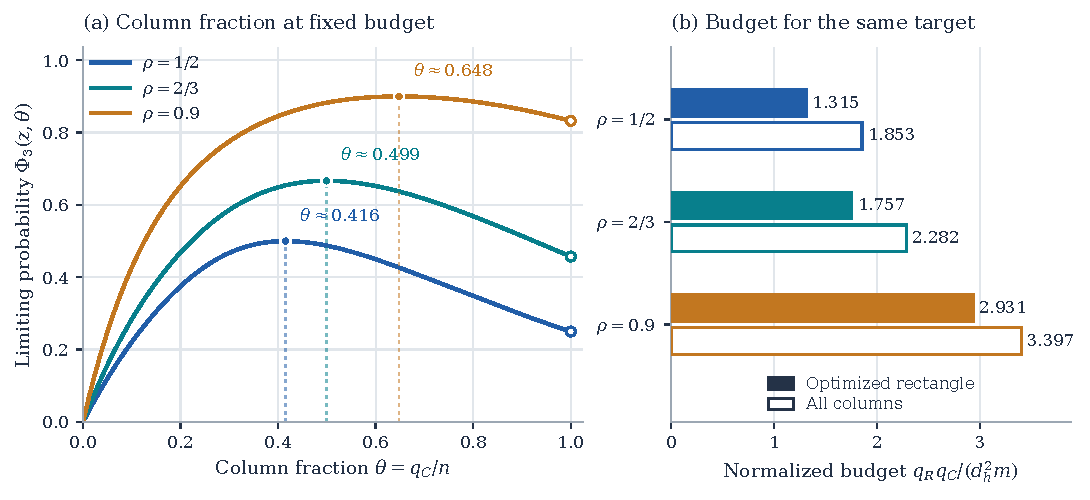
\includegraphics[width=\textwidth]{figures/rectangular_sampling.pdf}
\caption{The limiting detection law at three optimized budgets for
\(s=3\). Filled points mark numerically located maximizers; open
points show all-column sampling at the same budget. No uniqueness
claim is needed. The budget comparison uses the constants of
\cref{tab:rectangle-constants}. The theorem proves the variational
characterization; the plotted locations are numerical approximations.}
\label{fig:rectangular}
\end{figure}

Taking all columns already attains the optimal order
\(\Theta(d_h^2m)\); choosing an interior fraction improves its
constant. Balanced samples instead require
\(\Theta(d_h^2m^{4/3})\) entries at fixed positive detection
probability. The difference is substantial and follows from the
particular three-position witness structure.

\subsection{Scope of the one-sided testing conclusion}

The rows of \(H\) are pairwise distinct, and its columns are pairwise
distinct. This simple fact identifies the strongest possible one-sided
decision rule when the information is one sampled rectangle.

\begin{proposition}[Completion of a negative observation]
\label{prop:completion}
Fix row indices \(r_1<\cdots<r_a\) and column indices
\(c_1<\cdots<c_b\) in \([n]\), where \(a,b\ge1\). Every
\(H\)-free binary matrix \(B\) of size \(a\times b\) extends to
an \(H\)-free \(n\times n\) matrix agreeing with \(B\) at those
prescribed indices. Consequently, among one-sided algorithms observing
only this uniformly sampled rectangle, rejecting whenever a visible
\(H\)-copy occurs is optimal, even when the sampled indices are known.
\end{proposition}
\begin{proof}
Choose nondecreasing surjections \(f:[n]\to[a]\), \(g:[n]\to[b]\)
with \(f(r_i)=i\) and \(g(c_j)=j\); filling the gaps by repeated
neighboring values constructs them. Define
\(\widetilde B(x,y)=B(f(x),g(y))\).
If \(\widetilde B\) contained \(H\), two of its selected rows could
not have the same \(f\)-image: they would have identical traces on
the selected columns, whereas the rows of \(H\) are distinct.
The same holds for selected columns and \(g\). The images are
therefore strictly increasing and give an \(H\)-copy in \(B\), a
contradiction.

An observation with no visible copy is thus consistent with an
\(H\)-free input on precisely the same sampled indices. That sample
has positive probability under the uniform sampling rule. Rejecting
such an observation with positive conditional probability would
violate one-sided correctness on its free completion. The visible-copy
rule rejects every remaining observation and is therefore optimal.
\end{proof}

This proposition and \cref{thm:optimal-rectangle} concern fixed sizes
and one sampled rectangle. They do not determine the optimal query
complexity of arbitrary adaptive entry queries, several sampled
rectangles, or random mixtures of sampling budgets.

\section{Exact inverse logarithmic repair cost}
\label{sec:inversion}

\subsection{The combinatorial relation and its Lambert inverse}

In this section we return to the main pattern: \(s=3\),
\(d=20h+2\), and \(m=2^h\).
Normalize the original-copy transversal by the total number of cells:
\begin{equation}
 \tau_h=\frac{\tau_H(A_h)}{n^2}=\frac{1}{d^2m},\qquad
 \eps_h=\dist_H(A_h)=d^{-2},\qquad a=\frac{\log2}{20}.
 \label{eq:tau-definition}
\end{equation}
Since \(m=\exp(a(d-2))\), the exact relation is
\begin{equation}
 \tau_h=e^{2a}d^{-2}e^{-ad}
       =e^{2a}\eps_h\exp(-a\eps_h^{-1/2}).
 \label{eq:tau-epsilon}
\end{equation}
The total copy density also satisfies the exact identity
\(\delta_h=2\eps_h^3\tau_h^2\).

Let \(W_0\) denote the real principal Lambert function,
characterized on positive arguments by \(W_0(x)e^{W_0(x)}=x\).
\begin{proposition}[Exact inversion]
\label{prop:lambert}
For every \(\tau>0\), the relation
\(\tau=e^{2a}\eps\exp(-a\eps^{-1/2})\) has exactly one positive
solution \(\eps\), namely
\begin{equation}
 \eps(\tau)=
 \frac{a^2}{4W_0\!\left((a/2)e^a\tau^{-1/2}\right)^2}.
 \label{eq:lambert-inverse}
\end{equation}
It agrees with the actual repair distance at \(\tau=\tau_h\).
\end{proposition}
\begin{proof}
Put \(d=\eps^{-1/2}>0\). Taking square roots and rearranging gives
\[
 d e^{ad/2}=e^a\tau^{-1/2},\qquad
 \frac{ad}{2}e^{ad/2}=\frac a2e^a\tau^{-1/2}.
\]
The argument is positive, and \(x\mapsto xe^x\) is strictly
increasing for \(x>0\), proving both the formula and uniqueness.
\end{proof}

This is an application of the existing linear--logarithmic inversion
machinery in ProveIt. The theorem labeled \texttt{p0:thm:lambert-core}
in its transseries manuscript solves \(aX+b\log X=L\) with the
appropriate Lambert branch~\cite{ProveItLambert}. Its positive-parameter
algebraic inversion and uniqueness are also implemented in
\texttt{LinLogCoreInversion.lean}~\cite{ProveItLean}. The present
contribution is the exact combinatorial relation
\eqref{eq:tau-epsilon}, together with its application below and the
explicit convergent coefficient formula. The general Lambert inversion
itself is prior machinery, and no Lean verification of the new matrix
theorems is claimed.

\subsection{A convergent expansion with an explicit remainder}

For sufficiently small \(\tau>0\), define
\begin{equation}
 X=\log(1/\tau)+2\log a+2a,\qquad t=\log X.
 \label{eq:X-inverse}
\end{equation}
Taking logarithms in \eqref{eq:tau-epsilon} shows that
\(u=ad\) is the unique positive solution of
\begin{equation}
 u+2\log u=X.
 \label{eq:inverse-core}
\end{equation}

\begin{theorem}[Convergent logarithmic expansion]
\label{thm:convergent-inverse}
For every real \(X\ge64\), the repair-cost inverse has the absolutely
convergent expansion
\begin{equation}
 \eps(\tau)=\frac{a^2}{X^2}
 \left(1+\sum_{j\ge1}\frac{B_j(\log X)}{X^j}\right),
 \label{eq:convergent-inverse}
\end{equation}
where the rational polynomial \(B_j\) is
\begin{equation}
 B_j(t)=\frac{(-2)^{j+1}}{j!}
 \left.\frac{\dd^{j-1}}{\dd w^{j-1}}
    \frac{(t+\log(1+w))^j}{(1+w)^3}\right|_{w=0}.
 \label{eq:inverse-coefficients}
\end{equation}
It has degree \(j\) and leading coefficient \(2^j(j+1)\). The
first four polynomials are
\begin{align*}
 B_1(t)&=4t,\\
 B_2(t)&=12t^2-8t,\\
 B_3(t)&=32t^3-56t^2+16t,\\
 B_4(t)&=80t^4-\frac{752}{3}t^3+192t^2-32t.
\end{align*}
Put \(r_X=8(\log X+1)/X<1\). For every integer \(N\ge0\),
\begin{equation}
 \left|\eps(\tau)-\frac{a^2}{X^2}
  \left(1+\sum_{j=1}^{N}\frac{B_j(\log X)}{X^j}\right)\right|
 \le\frac{4a^2}{X^2}\frac{r_X^{N+1}}{1-r_X}.
 \label{eq:inverse-remainder}
\end{equation}
\end{theorem}
\begin{proof}
Write \(u=X(1+v)\), \(z=X^{-1}\), and \(t=\log X\). Equation
\eqref{eq:inverse-core} becomes
\begin{equation}
 v=-2z\bigl(t+\log(1+v)\bigr).
 \label{eq:inverse-fixed-point}
\end{equation}
For the moment hold \(t\ge0\) fixed, permit complex \(z\), use the
analytic logarithm on \(|v|<1\), and set \(R_t=1/[8(t+1)]\).
For \(|v|\le1/2\), the power series for the logarithm gives
\( |\log(1+v)|\le\log2<1\). Thus, when \(|z|\le R_t\), the
right side of \eqref{eq:inverse-fixed-point} has modulus at most
\[
 \frac{t+\log2}{4(t+1)}<\frac14,
\]
and its derivative in \(v\) has modulus at most
\(4|z|\le1/[2(t+1)]\le1/2\). Iteration from zero is a uniform
contraction on the closed disk \(|v|\le1/2\). Its analytic iterates
converge locally uniformly to a solution \(v(z,t)\), analytic for
\(|z|<R_t\), with \(|v|\le1/4\).

Apply Lagrange inversion to
\(F(w)=(1+w)^{-2}\) and \(\phi(w)=-2(t+\log(1+w))\):
\[
 [z^j]F(v(z,t))
 =\frac1j[w^{j-1}]F'(w)\phi(w)^j=B_j(t).
\]
For \(t>0\), the coefficient identity follows by changing variable
\(z=w/\phi(w)\) in the coefficient integral and integrating a
derivative; for \(t=0\), it follows by continuity, or directly from
\(v(z,0)=0\). Substituting \(F'\) and \(\phi\) gives
\eqref{eq:inverse-coefficients}. Finite differentiation gives the
displayed first terms. The coefficient of \(t^j\) is obtained from
\((1+w)^{-3}\), since
\[
 \left.\frac{\dd^{j-1}}{\dd w^{j-1}}(1+w)^{-3}\right|_{w=0}
 =(-1)^{j-1}\frac{(j+1)!}{2}.
\]
This yields \(2^j(j+1)\).

On the analytic solution disk, \(|F(v)|\le4\). Cauchy's estimate
on smaller radii and passage to \(R_t\) give
\[
 |B_j(t)|\le4R_t^{-j}=4[8(t+1)]^j.
\]
For \(X\ge64\), one has \(r_X<1\): the function
\(X-8\log X-8\) is increasing for \(X>8\) and positive at
\(64\), using \(\log64=6\log2<6\). Thus \(z=1/X<R_t\),
and the series converges absolutely. The real fixed point satisfies
\(u=X(1+v)>0\). Because \(u+2\log u\) increases from
\(-\infty\) to \(+\infty\), this is the unique solution in
\eqref{eq:inverse-core}. The identity \(\eps=a^2/u^2\) proves
\eqref{eq:convergent-inverse}.

Finally, the coefficient bound gives
\[
 \left|\sum_{j>N}B_j(\log X)X^{-j}\right|
 \le4\sum_{j>N}r_X^j=4\frac{r_X^{N+1}}{1-r_X}.
\]
Multiplication by \(a^2/X^2\) proves the explicit remainder estimate.
\end{proof}

\subsection{A necessary barrier for repair from existing-copy covers}

In particular,
\begin{equation}
 \eps_h\sim\frac{a^2}{\log^2(1/\tau_h)}.
 \label{eq:logarithmic-barrier}
\end{equation}
This is a constraint on any putative universal conversion from the
size of an existing-copy transversal to the size of a successful
binary repair.

\begin{corollary}[Inverse logarithmic obstruction]
\label{cor:inverse-barrier}
Suppose a function \(\Psi:[0,1]\to[0,1]\) satisfies
\[
 \dist_H(A)\le\Psi\!\left(\frac{\tau_H(A)}{n^2}\right)
\]
for every binary \(n\times n\) matrix \(A\). Then
\(\Psi(\tau_h)\ge\eps(\tau_h)\), with the exact inverse and
expansion above. In particular \(\Psi(t)=o(\log^{-2}(1/t))\) as
\(t\downarrow0\) is impossible. If \(\Psi\) is nondecreasing, then
\begin{equation}
 \liminf_{t\downarrow0}\Psi(t)\log^2(1/t)\ge a^2.
 \label{eq:all-t-barrier}
\end{equation}
\end{corollary}
\begin{proof}
Apply the proposed bound to \(A_h\) and use the exact formulas.
For the last assertion, choose \(h\) with
\(\tau_{h+1}\le t\le\tau_h\). Monotonicity gives
\(\Psi(t)\ge\eps_{h+1}\). Also
\[
 \log(1/\tau_{h+1})-\log(1/\tau_h)
 =\log2+2\log\left(\frac{d_h+20}{d_h}\right)=\log2+o(1).
\]
The logarithmic mesh is bounded, so \eqref{eq:logarithmic-barrier}
at \(h+1\) gives \eqref{eq:all-t-barrier}.
\end{proof}

The corollary supplies a necessary lower bound on such a conversion
function. It does not prove a matching universal upper bound for
arbitrary ordered matrices; that remains a separate structural question.
